\chapter{Funções de Mão Única*}
\label{cha:owf}

Nos Capítulos \ref{cha:cifras-de-fluxo}, \ref{cha:cifras-de-bloco} e \ref{cha:mac} demonstramos que dadas certas suposições determinados sistemas de criptografia garantem a segurança contra determinados modelos de ataque.
Argumentamos que essas supoções -- a saber, a existência de geradores de números pseudoaleatórios, de funções pseudoaleatórias e de permutações pseudoaleatórias -- não são provadas, mas validadas empiricamente.
Neste capítulo argumentaremos porque não construimos sistemas que comprovadamente satisfazem essas suposições.
Para tanto apresentaremos uma condição necessária e suficiente para a existência de sistemas seguros: a existência de funções de mão única.
Por fim mostraremos que uma demonstração da existência de funções de mão única implicam que $P \neq NP$, ou seja, esse resultado teria como consequência um dos problemas em aberto mais relevantes na matemática hoje.

Uma {\em função de mão única} é uma função $f: \{0,1\}^n \to \{0,1\}^n$ que pode ser computada de maneira eficiente, mas que é inviável de ser invertida.
Ou seja, para todo adversário eficiente $\mathcal{A}$ que recebe $y := f(x)$ só consegue encontrar $x'$ tal que $f(x') = y$ com probabilidade desprezível \cite{Diffie76,Yao82}.

Formalmente definimos função de mão única por meio do seguinte jogo:
\begin{enumerate}
\item O sistema escolhe $x \leftarrow \{0,1\}^n$ e computa $y := f(x)$.
\item O adversário $\mathcal{A}$ recebe $1^n$ e $y$.
\item $\mathcal{A}$ devolve $x' \in \{0,1\}^n$.
\end{enumerate}

O desafio do adversário é produzir uma pré-imagem de $f$, ou seja, um $x'$ tal que $f(x') = y$:

\begin{displaymath}
  Inv_{\mathcal{A}, f}(n) := \left\{
    \begin{array}{lcl}
      1 & \textrm{se} & f(x') = y\\
      0 & \textrm{c.c.} &\\
    \end{array}
    \right.
\end{displaymath}

Uma função $f: \{0,1\}^n \to \{0,1\}^n$ é de mão única se:
\begin{enumerate}
\item $f$ pode ser computada de maneira eficiente (polinomial) e
\item Para todo adversário eficiente $\mathcal{A}$ existe $\varepsilon$ desprezível tal que:
\begin{displaymath}
  Pr[Inv_{\mathcal{A}, f}(n) = 1] \leq \varepsilon(n)
\end{displaymath}
\end{enumerate}


\begin{example}
  Uma candidata a função de mão é única é a seguinte função para $x$ e $y$ de mesmo tamanho e primos:
  \begin{displaymath}
    f(x,y) := x \cdot y
  \end{displaymath}
  A dificuldade de inverter $f$ está a associada ao {\em problema da fatoração} que é considerado um problema difícil.

  Veremos no Capítulo \ref{cha:distribuicao-chaves} que para certos grupos $G$ com gerador $g$ temos que a seguinte função $f$ é de mão única:
  \begin{displaymath}
    f_g(x) := g^x
  \end{displaymath}

A dificuldade de inverter esta função está associada ao chamado {\em problema do logarítmo discreto}.
\end{example}


Note que para derrotar o desafio de uma função de mão única $\mathcal{A}$ precisa calcular a pré-imagem $x'$, não basta conhecer alguma informação parcial sobre $x'$.
Um {\em predicado hard-core} é um bit de informação sobre a $x'$ que é mantido escondido pela função de mão única $f$ \cite{Blum84}.
Formalmente, um predicado hard core é uma função $hc:\{0,1\}^n \to \{0,1\}$ se qualquer adversário eficiente que conhece $y := f(x)$ consegue acertar o valor de $hc(x)$ apenas com change desprezivelmente maior do que $\frac{1}{2}$.


Seja $f:\{0,1\}^n \to \{0,1\}^n$ uma função de mão única.
Considere a função $g(x,r) := \langle f(x), r \rangle$ em que $|x| = |r|$ e defina $hc(x,r) := \bigoplus_{i=1}^nx_i \cdot r_i$.
É possível mostrar que $g$ é uma função de mão única e $hc$ é um predicado hard-core de $g$ \cite{Goldreich89}.
Esta construção é a base do seguinte teorema\footnote{Neste capítulo seguiremos essa abordagem de apresentar as construções e omitir as demonstrações. O leitor interessado deve procurar o livro do Goldreich \cite{Goldreich07} para uma apresentação completa sobre os temas tratados neste capítulo.}:

\begin{theorem}[Goldreich-Levin]
  Assuma que uma função de mão única existe. Então existe uma função de mão única com um predicado hard-core.
\end{theorem}

Uma vez extraído um bit ``seguro'' a partir de uma função de mão única, podemos usá-lo na construção de um PRG com fator de expanção $l(n) = n + 1$.

\begin{theorem}
  Seja $f$ uma função de mão única com um predicado hard-crore $hc$.
A função $G(s) := f(s)||hc(s)$ é um PRG com fator de expansão $l(n) = n+1$.
\end{theorem}

Agora que somos capazes de gerar um PRG com fator de expansão mínimo, é possível expandi-lo para um PRG com fator de expansão $l(n) = p(n)$ em que $p$ é um polinomio qualquer.
Seja $G$ um PRG com fator de expansão mínimo, construimos $G'$ da seguinte maneira.
Usamos $G$ para gerar $l(n)+1$ bits, o último bit é usado como primeiro bit da sáida de $G'$ e os demais são usados como uma nova semente para $G$ e repetimos o processo quantas vezes forem nescessárias.
Esta construção é a base do seguinte teorema:


\begin{theorem}
  Se existe PRG com fator de expansão $l(n) = n + 1$ então para todo polinômio $p$ existe PRG $G'$ com fator de expansão $l(n) = p(n)$.
\end{theorem}

\begin{figure}[htbp]
  \centering
    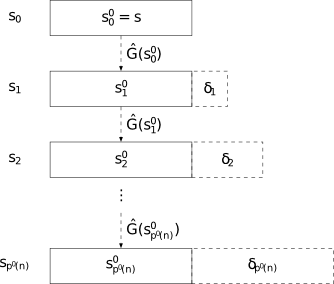
\includegraphics[width=.5\textwidth]{imagens/OWF-PRG.png}
  \caption{Diagrama da construção de $G'$}
  \label{fig:owf-prg}
\end{figure}
% Este diagrama está ruim!!

É possível construir uma função pseudoaleatória a partir de um PRG com fator de expansão $2n$.
Seja $G(k) = y_0 \dots y_{2n}$ um PRG e defina $G_0(k) := y_0 \dots y_n$ e $G_1(k) := y_{n+1} \dots y_{2n}$.
Construiremos uma PRF $f_k: \{0,1\}^n \to \{0,1\}^n$ da seguinte maneira:
\begin{displaymath}
  f_k(x_1 \dots x_n) := G_{x_n}(\dots (G_{x_1}(k))\dots)
\end{displaymath}

\begin{theorem}[Yao]
  Se $G$ é um PRG com fator de expansão $l(n) = 2n$ então a construção acima é um PRF.  
\end{theorem}

\begin{figure}[htbp]
  \centering
    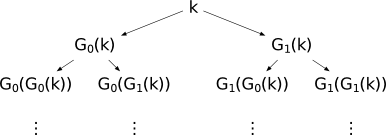
\includegraphics[width=.7\textwidth]{imagens/PRG-PRF.png}
  \caption{Construção de Yao}
  \label{fig:owf-prg}
\end{figure}

Para completar, a partir de uma PRF é possível construir uma PRP usando uma rede de Feistel com três passos em que cada passo usa uma chave distinta.
\begin{displaymath}
  f_{k_1,k_2,k_3}^{(3)}(x) := Feistel_{f_{k_1},f_{k_2},f_{k_3}}(x)
\end{displaymath}
Lembrando que:

\begin{eqnarray*}
  Feistel_{f_1,\dots,f_n}(x) & := & L_nR_n\\
  L_i & := & R_{i-1}\\
  R_i & := & L_{i-1} \xor f_i(R_{i-1})
\end{eqnarray*}


\begin{theorem}
  Se $f$ é uma PRF então $f^{(3)}$ é uma permutação pseudoaleatória.
\end{theorem}

% DIAGRAMA DA CONSTRUÇÃO DE F3

Resumindo, a existência de uma função de mão única é uma condição suficiente para a existência de PRG, PRF e PRP.
No Capítulos \ref{cha:cifras-de-fluxo} vimos que a existência de um PRG é condição suficiente para construir um sistema seguro contra ataques {\em ciphertext only} e nos Capítulos \ref{cha:cifras-de-bloco} e \ref{cha:mac} vimos que a existência de uma PRF é condição suficiente para construção de sistemas de criptografia seguros contra CPA e contra CCA, bem como para construção de sistemas autenticados.

O teorema a seguir mostra a condição reversa, ou seja, que a existência de função de mão única é condição necessária para existência de todas essas construções:


\begin{theorem}
  Se existe um sistema seguro contra ataques {\em ciphertext only} que protega uma mensagem duas vezes maior do que sua chave então existe uma função de mão única.
\end{theorem}

\begin{proof}
Seja $\Pi = \langle Gen, E, D \rangle$ um sistema de criptografia seguro contra ataques ``ciphertext only''.
Seja $|k| = n$, $|m| = 2n$ e $r$ os bits aleatórios usados em $E$ (nos casos que vimos seria o IV) com $|r| = l(n)$ onde $l$ é um polinômio qualquer.
Construímos uma função da seguinte forma:
\begin{displaymath}
  f(k, m, r) := E(k, m||r)||m
\end{displaymath}

Vamos mostrar que $f$ é uma função de mão única.
Seja $\mathcal{A}$ um adversário para o problema de inverter $f$.
Vamos construir $\mathcal{A}'$ um adversário para $\Pi$ da seguinte forma:
\begin{enumerate}
\item Escolhe $m_0, m_1 \leftarrow \{0,1\}^{2n}$ e devolve $c$
\item Roda $\mathcal{A}(c||m_0)$ para obter $k'$, $m'$ e $r'$.
Se $f(k', m', r') = c ||m_0$ devolve $0$, se não devolve $1$.
\end{enumerate}
 
Note que se $E(k,m_0) = c$ então $c||m_0$ tem distribuição identica a $f(k, m_0, r)$.
Portanto, temos que $\mathcal{A}'$ perde o jogo com probabilidade $Pr[Inv_{\mathcal{A}, f}(n) = 1]$.
Por outro lado se $E(k, m_1) = c$ então $c$ é independente de $m_0$ e portanto a probabilidade de $D(k, c) = m_0 $ é $\frac{2^n}{2^{2n}} = 2^{-n}$.
Temos então o seguinte:


\begin{eqnarray*}
  Pr[PrivK_{\Pi, \mathcal{A}'}^{eav}(n) = 1] & = & \frac{Pr[\mathcal{A}' = 0 | b = 0]}{2} + \frac{Pr[\mathcal{A}' = 1 | b = 1]}{2}\\
  & \geq & \frac{Pr[Inv_{\mathcal{A},f}(n) = 1]}{2} + \frac{1 - 2^{-n}}{2}\\
  & = & \frac{1}{2} + \frac{Pr[Inv_{\mathcal{A},f}(n) = 1] - 2^{-n}}{2}
\end{eqnarray*}

Nossa suposição de que $\Pi$ é seguro contra ataques do tipo ``chosen plaintext'' implica que existe $\varepsilon$ desprezível tal que $Pr[PrivK_{\Pi, \mathcal{A}'}^{eav}(n) = 1] \leq \frac{1}{2} + \varepsilon(n)$ e portanto:

 \begin{eqnarray*}
  \frac{1}{2} + \frac{Pr[Inv_{\mathcal{A},f}(n) = 1] - 2^{-n}}{2} & \leq & \frac{1}{2} + \varepsilon(n)\\
  \frac{Pr[Inv_{\mathcal{A},f}(n) = 1] - 2^{-n}}{2} & \leq & \varepsilon(n)\\
  Pr[Inv_{\mathcal{A},f}(n) = 1] & \leq & 2\varepsilon(n) + 2^{-n}\\
\end{eqnarray*}

Como $2\varepsilon(n) + 2^{-n}$ é desprezível, concluímos que $f$ é uma função de mão única.

\end{proof}

\begin{figure}[htbp]
  \centering
    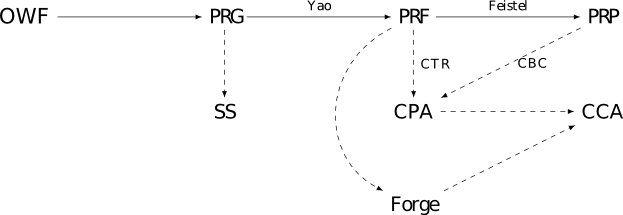
\includegraphics[width=.7\textwidth]{imagens/OWF-diagrama.png}
  \caption{Cadeia de consequências da existência de funções de mão única}
  \label{fig:owf-seguranca}
\end{figure}

Acreditamos que certas função são de mão única, hipótese esta que é validada empiricamente.
Porém, não temos uma demonstração matemática desta afirmação.
Suponha que conseguissemos mostrar que $f$ é uma função de mão única.
Por definição temos que $f(x)$ deve ser computável em tempo polinomial.
Se sabemos que $f^{-1}(x) = y$ então podemos verificar isso em tempo polinomial testando se $f(y) = x$.
Em outras palavras, $f$ é um oráculo polinomial para $f^{-1}$, ou seja, $Inv_f(n) \in NP$.
A definiçao de função de mão única estabelece que $Inv_f(n) \notin P$.
Portanto, se existe uma função de mão única temos que $P \neq NP$.
A relação entre os problemas polinomais $P$ e os problemas para os quais existe um oráculo polinomial $NP$ é o problema em aberto mais importante na ciência da computação e um dos mais importantes em aberto na matemática.

\section{Exercícios}
\label{sec:exercicios}

\begin{exercicio}
  Mostre que $f(x,y) = x \cdot y$ sem as restrições de que $x$ e $y$ sejam primos e do mesmo tamanho não é uma função de mão única.
\end{exercicio}


\begin{exercicio}
  Mostre um grupo cíclico com gerador $g$ (ver Capítulo \ref{cha:distribuicao-chaves}) em que $f_g(x) = g^x$ não é uma função de mão única.
\end{exercicio}
